\begin{filecontents*}{references.bib}
@inproceedings{ave2026,
  author = {Ave, Jonas and Pekaric, Irdin and Frohner, Matthias and Apruzzese, Giovanni},
  title = {{``bot lane noob'': Towards Practical Deployment of NLP-based Toxicity Detectors in Video Games}},
  booktitle = {European Symposium on Research in Computer Security (ESORICS)},
  year = {2026},
  note = {Forthcoming}
}

@misc{jigsaw,
  author = {{Jigsaw} and {Google}},
  title = {Toxic Comment Classification Challenge},
  year = {2018},
  howpublished = {\url{https://www.kaggle.com/competitions/jigsaw-toxic-comment-classification-challenge}},
  note = {Kaggle}
}

@inproceedings{davidson2017,
  author = {Davidson, Thomas and Warmsley, Dana and Macy, Michael and Weber, Ingmar},
  title = {Automated Hate Speech Detection and the Problem of Offensive Language},
  booktitle = {Proceedings of the Eleventh International AAAI Conference on Web and Social Media (ICWSM)},
  year = {2017},
}

@inproceedings{kwak2015,
  author = {Kwak, Haewoon and Blackburn, Jeremy and Han, Seungyeop},
  title = {Exploring Cyberbullying and Other Toxic Behavior in Team Competition Online Games},
  booktitle = {Proceedings of the 33rd Annual ACM Conference on Human Factors in Computing Systems (CHI)},
  year = {2015},
  doi = {10.1145/2702123.2702529}
}

@inproceedings{toxic_chat_rg,
  author = {Lee, Jaehong and Rerkjirattikal, Pavinee and Nam, Sanggyu},
  title = {Toxic Chat Detection in Online Games Using Hybrid {BERT} and Character-level {CNN}},
  booktitle = {Proceedings of the MakeLearn, TIIM \& PIConf International Conference},
  year = {2025},
  address = {Bangkok, Thailand}
}

@article{hochreiter1997,
  author = {Hochreiter, Sepp and Schmidhuber, J\"{u}rgen},
  title = {Long Short-Term Memory},
  journal = {Neural Computation},
  volume = {9},
  number = {8},
  year = {1997}
}
\end{filecontents*}

\documentclass[final]{article}

% aps360 loads natbib; force numerical cites to match IEEEtran.bst.
% [main] defines \@trackname required by the [final] footer notice.
\PassOptionsToPackage{numbers,sort&compress}{natbib}
\usepackage[main]{aps360}
\usepackage[utf8]{inputenc} % allow utf-8 input
\usepackage[T1]{fontenc}    % use 8-bit T1 fonts
\usepackage{hyperref}       % hyperlinks
\usepackage{url}            % simple URL typesetting
\usepackage{booktabs}       % professional-quality tables
\usepackage{amsmath}        % \mathrm and related math helpers
\usepackage{amsfonts}       % blackboard math symbols
\usepackage{nicefrac}       % compact symbols for 1/2, etc.
\usepackage{microtype}      % microtypography
\usepackage{xcolor}         % colors
\usepackage{graphicx}       % figures
\usepackage{caption}        % consistent caption spacing / alignment
\captionsetup{
  justification=centering,
  singlelinecheck=false,
  skip=10pt,
  position=bottom
}
\setlength{\abovecaptionskip}{10pt}
\setlength{\belowcaptionskip}{2pt}
\setlength{\intextsep}{6pt}
\setlength{\textfloatsep}{6pt}
\setlength{\floatsep}{6pt}
% Frozen development-set metrics (from reports/progress; regenerate via generate_report_assets.py).
\newcommand{\BaselineValidationFOne}{0.629}
\newcommand{\BaselineAccuracy}{0.927}
\newcommand{\BaselineBalancedAccuracy}{0.849}
\newcommand{\BaselinePrecision}{0.579}
\newcommand{\BaselineRecall}{0.754}
\newcommand{\BaselineFOne}{0.655}
\newcommand{\BaselineTruePositives}{147}
\newcommand{\BaselineFalsePositives}{107}
\newcommand{\LSTMAccuracy}{0.938}
\newcommand{\LSTMBalancedAccuracy}{0.781}
\newcommand{\LSTMPrecision}{0.688}
\newcommand{\LSTMRecall}{0.590}
\newcommand{\LSTMFOne}{0.634}
\newcommand{\LSTMFOneStd}{0.015}
\newcommand{\BaselineMinusLSTMFOne}{0.021}
\newcommand{\LSTMEnsembleFOne}{0.644}
\newcommand{\LSTMValidationFOne}{0.648}
\newcommand{\LSTMValidationFOneStd}{0.015}
\newcommand{\LSTMSeedFortyTwoFOne}{0.619}
\newcommand{\LSTMTruePositives}{117}
\newcommand{\LSTMFalsePositives}{66}
\newcommand{\LSTMThreshold}{0.90}
\newcommand{\LSTMBestEpoch}{5}
\newcommand{\LSTMParameters}{612,885}
\newcommand{\LSTMVocabSize}{3,629}
\newcommand{\LSTMHiddenDimension}{128}
\newcommand{\LSTMLayers}{2}
\newcommand{\LSTMDropout}{0.3}
\newcommand{\PreparedRows}{14,293}
\newcommand{\HybridAccuracy}{0.945}
\newcommand{\HybridBalancedAccuracy}{0.793}
\newcommand{\HybridPrecision}{0.748}
\newcommand{\HybridRecall}{0.609}
\newcommand{\HybridFOne}{0.666}
\newcommand{\HybridFOneStd}{0.015}
\newcommand{\HybridMinusBaselineFOne}{0.012}
\newcommand{\HybridValidationFOne}{0.671}
\newcommand{\HybridValidationFOneStd}{0.007}
\newcommand{\HybridSeedFortyTwoFOne}{0.680}
\newcommand{\HybridTruePositives}{133}
\newcommand{\HybridFalsePositives}{63}
\newcommand{\HybridThreshold}{0.60}
\newcommand{\HybridAlphaSeedFortyTwo}{0.3}
\newcommand{\HybridAlphas}{0.3, 0.0, 0.6}
\newcommand{\HybridThresholds}{0.60, 0.60, 0.80}
\newcommand{\HybridBestEpoch}{5}
\newcommand{\HybridParameters}{612,885}
\newcommand{\HybridVocabSize}{3,629}
\newcommand{\HybridHiddenDimension}{128}
\newcommand{\HybridLayers}{2}
\newcommand{\HybridDropout}{0.3}
\newcommand{\ContextBestValidationFOne}{0.633}

% Locked fresh final test (artifacts/final_test/final_test_metrics.json).
\newcommand{\FreshMessages}{332}
\newcommand{\FreshMatches}{14}
\newcommand{\FreshToxic}{49}
\newcommand{\FreshNonToxic}{283}
\newcommand{\FreshToxicPrevalence}{14.8\%}
\newcommand{\FreshBaselineAccuracy}{0.837}
\newcommand{\FreshBaselineBalancedAccuracy}{0.660}
\newcommand{\FreshBaselinePrecision}{0.444}
\newcommand{\FreshBaselineRecall}{0.408}
\newcommand{\FreshBaselineFOne}{0.426}
\newcommand{\FreshLSTMAccuracy}{0.834}
\newcommand{\FreshLSTMBalancedAccuracy}{0.582}
\newcommand{\FreshLSTMPrecision}{0.393}
\newcommand{\FreshLSTMRecall}{0.224}
\newcommand{\FreshLSTMFOne}{0.286}
\newcommand{\FreshHybridAccuracy}{0.855}
\newcommand{\FreshHybridBalancedAccuracy}{0.620}
\newcommand{\FreshHybridPrecision}{0.519}
\newcommand{\FreshHybridRecall}{0.286}
\newcommand{\FreshHybridFOne}{0.368}
\newcommand{\FreshTrueNegatives}{270}
\newcommand{\FreshFalsePositives}{13}
\newcommand{\FreshFalseNegatives}{35}
\newcommand{\FreshTruePositives}{14}
\newcommand{\FreshAllSafeAccuracy}{0.852}
\newcommand{\FreshSVMLiftOverHybridFOne}{0.057}
\newcommand{\FreshHybridSeedFortyTwoFOneDrop}{0.312}


\title{LoL Toxic Gaming Chat Classifier: Final Report}

\author{%
  Alex You \\
  1011175185, alex.you@mail.utoronto.ca\\
  \href{https://github.com/youalex018/aps360-final-project}{Link to GitHub repository}\\
}

\begin{document}

\maketitle

\vspace{-0.5in}

\section*{Introduction}

Chat in competitive multiplayer games like League of Legends (LoL) is short, slang-heavy, and hard for generic toxicity filters to handle. Phrases like ``inting'' (intentionally feeding) or ``bot diff'' (blaming bot lane) are common. This project classifies one raw chat line as toxic or non-toxic. Machine learning fits because tone depends on context: a sincere ``nice'' is fine, but ``nice play'' can be sarcasm. I compare a TF--IDF (term frequency--inverse document frequency, a word-importance weighting) + linear SVM (support vector machine) baseline, an LSTM (long short-term memory) sequence model \cite{hochreiter1997}, and a late-fusion hybrid that blends the two models' scores after each runs independently. The hybrid is my primary model because many lines are only one or two tokens, so lexical cues still help. The problem is tough: labels are scarce and about 9\% toxic, messages are tiny, and Riot APIs do not expose chat, so I built a passive OCR (optical character recognition) collector that reads fresh live matches I play myself.

\section*{Illustration}

Figure~\ref{fig:overview} is the full pipeline: clean a message, score it with the LSTM and the SVM, fuse the scores, and decide toxic or non-toxic. Development uses the expert-labelled L2DTnH corpus \cite{ave2026}. Final testing uses two locked OCR collections from my own live matches, Batch~A and Batch~B, described under Evaluate Model on New Data.

\begin{figure}[!ht]
  \centering
  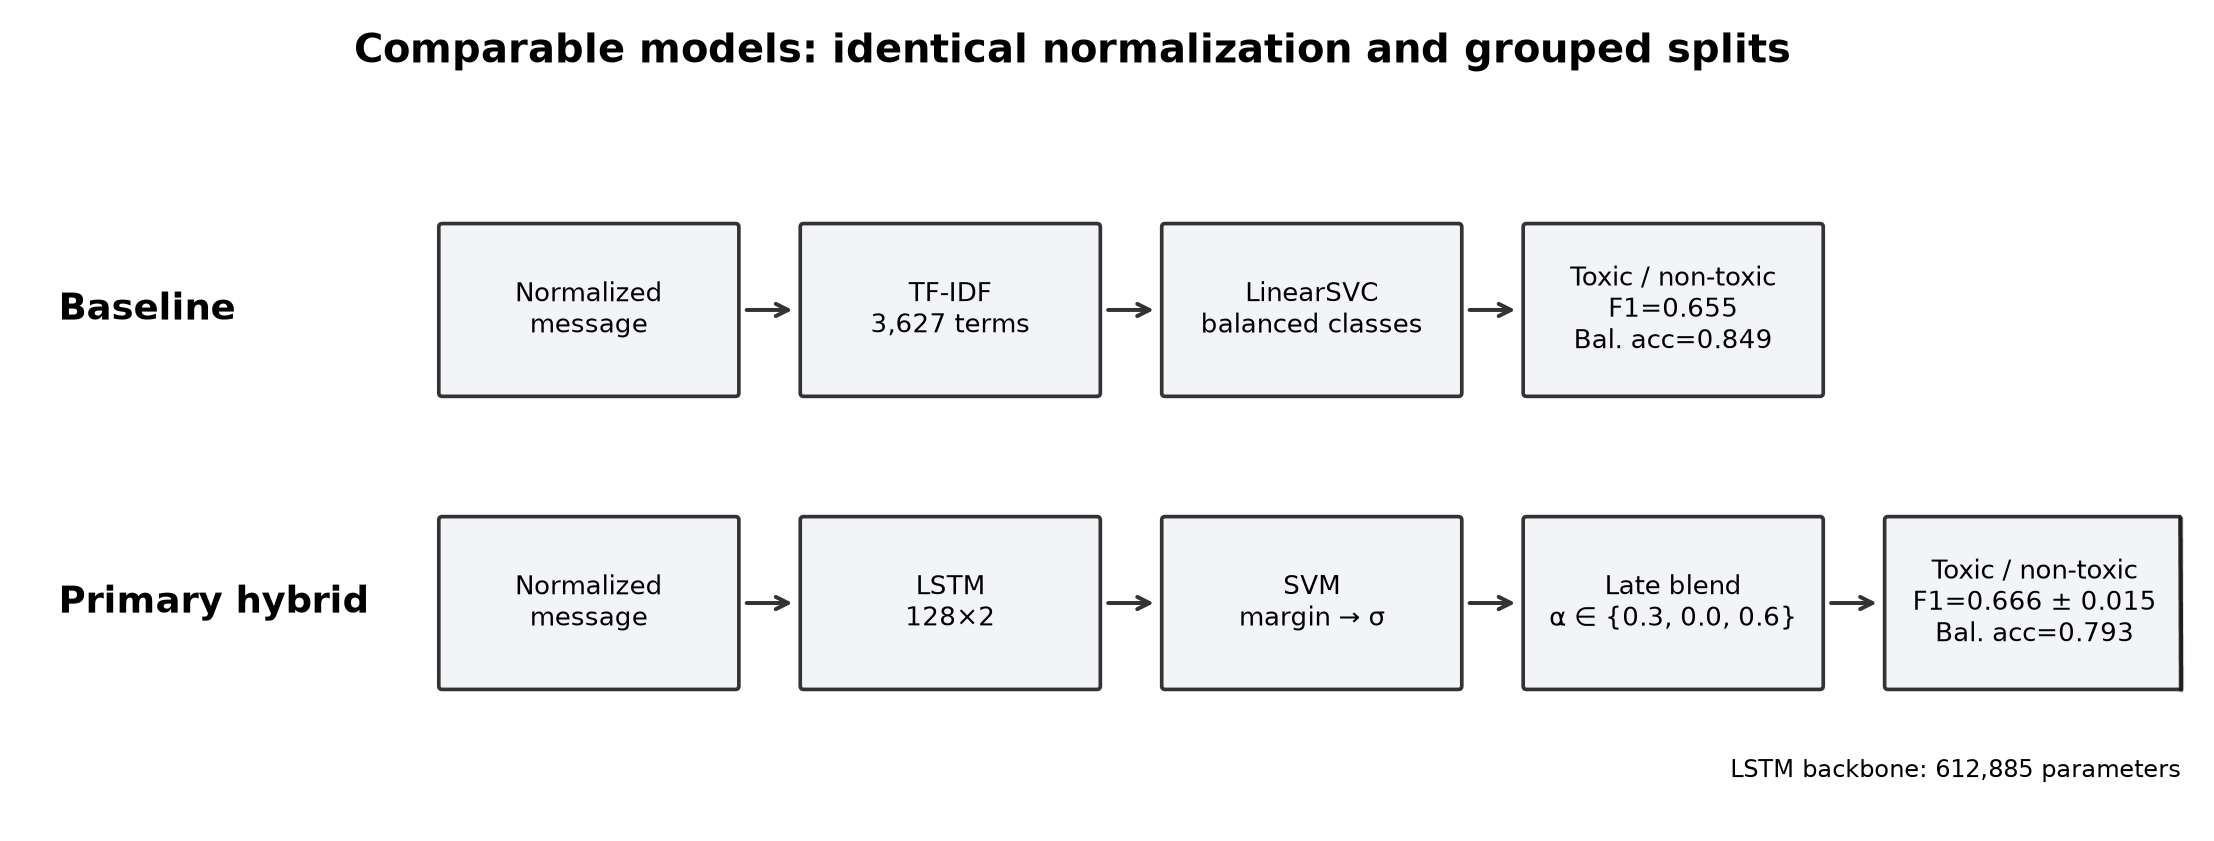
\includegraphics[width=0.90\textwidth]{architecture_comparison.png}
  \caption{Primary late-fusion hybrid: cleaned LoL chat $\rightarrow$ LSTM probability and SVM margin $\rightarrow$ fused toxic / non-toxic decision.}
  \label{fig:overview}
\end{figure}

\section*{Background \& Related Work}

Toxicity work on the internet is large. The Jigsaw Toxic Comment Challenge \cite{jigsaw} showed that models trained on general internet text need domain adaptation. Davidson et al.\ \cite{davidson2017} separate offensive language from targeted hate, which matters when deciding how harsh LoL ``toxicity'' should be. Kwak et al.\ \cite{kwak2015} look at toxic behaviour in team games like LoL and argue for domain-specific tools. For modelling, Hochreiter and Schmidhuber's LSTM \cite{hochreiter1997} is a solid short-text encoder when transformers are out of scope, and hybrid BERT + character-CNN work on game chat \cite{toxic_chat_rg} supports mixing lexical and neural cues. Closest to this project, Ave et al.\ release the L2DTnH dataset with message-level expert labels for LoL chat \cite{ave2026}. I train on that corpus and add a late-fusion SVM branch because a single-message LSTM alone loses to bag-of-words on ultra-short lines.

\section*{Data Processing}

I use L2DTnH, which has message-level labels from eight experienced LoL players \cite{ave2026}. Cleaning decodes HTML, normalizes Unicode, lowercases, collapses spaces, keeps alphanumeric tokens, and expands common slang (e.g., \texttt{ff} $\rightarrow$ ``forfeit''). I drop incomplete rows, empty messages, and texts with conflicting expert labels, but I keep repeated same-label lines because spam can itself be toxic. Instead of shuffling rows, I assign each full match to train / validation / test in about a 70/15/15 split so one game never crosses partitions and the toxic rate stays near 9\%.

\begin{table}[!ht]
\centering
\small
\setlength{\tabcolsep}{5pt}
\begin{minipage}[t]{0.58\linewidth}
  \centering
  \begin{tabular}{lrrrr}
  \toprule
  Partition & Messages & Non-toxic & Toxic & Chat logs \\
  \midrule
  Train & 10,050 & 9,123 & 927 & 70 \\
  Validation & 2,109 & 1,911 & 198 & 15 \\
  Test & 2,134 & 1,939 & 195 & 16 \\
  \bottomrule
  \end{tabular}
\end{minipage}
\hfill
\begin{minipage}[t]{0.38\linewidth}
  \centering
  \begin{tabular}{ll}
  \toprule
  Raw message & Cleaned tokens \\
  \midrule
  \texttt{its gg} & \texttt{its good game} \\
  \texttt{gold - elo} & \texttt{gold elo} \\
  \texttt{gj} & \texttt{good job} \\
  \bottomrule
  \end{tabular}
\end{minipage}
\caption{Grouped split and cleaned samples. \PreparedRows{} messages kept (1,320 toxic); median length is two tokens. ``Chat logs'' counts the distinct matches contributing to that partition.}
\label{tab:data}
\end{table}

\section*{Architecture}

For Batch~A, I froze a late-fusion hybrid of the LSTM with toxic class weight 7 and a word-level TF--IDF SVM (Figure~\ref{fig:overview}). After Batch~A failed, I screened character $n$-grams on the lexical branch using validation only. Selecting the fusion weight and threshold by F2 (more weight on recall) raised recall but dropped mean validation toxic F1 to 0.614, under my 0.671 freeze gate. The same character features with ordinary F1 selection hit mean validation F1 0.688, so I froze that character-$n$-gram hybrid for Batch~B.

\begin{itemize}
  \setlength{\itemsep}{0.1em}
  \setlength{\parsep}{0pt}
  \item \textbf{Input / embedding:} cleaned message, truncated or padded to 50 tokens; 100-D embeddings; vocab \HybridVocabSize{} (train only)
  \item \textbf{LSTM:} \HybridLayers{} layers, hidden \HybridHiddenDimension{}, dropout \HybridDropout; last time step; \HybridParameters{} parameters
  \item \textbf{Training:} Adam (lr $10^{-3}$), batch 64, toxic class weight 7, early stop on validation toxic F1 (patience 3)
  \item \textbf{SVM branch (Batch~B):} word TF--IDF plus character $n$-grams of length 3--5, then LinearSVC (fit on train only)
  \item \textbf{Fusion:} $\alpha\,p_{\mathrm{LSTM}}+(1-\alpha)\sigma(\mathrm{margin}_{\mathrm{SVM}})$, where $\sigma$ is a sigmoid that squashes the SVM's unbounded margin into a $[0,1]$ range comparable to the LSTM's probability; Batch~A freeze $\alpha=0.3$, threshold $0.60$; Batch~B freeze $\alpha\in\{0.2,0.0,0.0\}$, thresholds $\in\{0.60,0.55,0.55\}$
\end{itemize}

On validation I also tried stronger regularization, a smaller LSTM, a bidirectional LSTM, same-match context windows ($K=1,2,3$), and raising the vocabulary minimum count so rare tokens map to a shared unknown token. The single-message hybrid still won (val F1 \HybridValidationFOne$\pm$\HybridValidationFOneStd), and context alone peaked at validation F1 \ContextBestValidationFOne. More architecture searching did not beat late fusion of the simple LSTM with a strong lexical SVM. Figure~\ref{fig:curves} shows the seed-42 LSTM backbone curves: validation toxic F1 peaks at epoch \HybridBestEpoch{}, while train loss keeps falling.

\section*{Baseline Model}

The baseline is a bag-of-words classifier using the same cleaning function and match-grouped train / validation / test splits as the neural models. On train text only, a \texttt{TfidfVectorizer} turns each cleaned message into sparse word TF--IDF features, then a \texttt{LinearSVC} with \texttt{class\_weight=balanced} separates toxic from non-toxic; other hyperparameters stay at library defaults. I report toxic-class F1 on validation (\BaselineValidationFOne) without touching test. Only about 9\% of messages are toxic, so raw accuracy can look fine while missing many toxic lines; I emphasize toxic F1 and balanced accuracy instead. If this fast SVM already does well, the LSTM has to beat it on the same data, not just look more complicated.

\section*{Quantitative Results}

Table~\ref{tab:results} shows accuracy, balanced accuracy, and toxic-class precision / recall / F1 on the held-out development test and on locked fresh Batch~A. Toxic F1 (harmonic mean of precision and recall on the toxic class) is the score I care about most. On development, the hybrid reaches mean toxic F1 \HybridFOne$\pm$\HybridFOneStd across three seeds, a bit above the SVM (\BaselineFOne) and the LSTM alone (\LSTMFOne$\pm$\LSTMFOneStd); one seed even chose $\alpha=0$ (pure SVM), so the win is small, not large. On Batch~A the story flips: hybrid toxic F1 falls to \FreshHybridFOne{}, under the SVM's \FreshBaselineFOne{}, with recall only \FreshHybridRecall{} (14 of 49 toxic lines). As a post-hoc check on Batch~A only (not used to re-tune), ROC-AUC was 0.690 / 0.700 / 0.681 for hybrid / LSTM / SVM, meaning the model still ranks toxic messages above non-toxic ones better than chance. However, even an oracle hybrid threshold (the best possible cutoff chosen in hindsight, which a real deployment could never pick in advance) would only reach F1 0.434 versus the frozen 0.368. The gap between those two numbers is small, so the failure looks like missing vocabulary rather than a badly chosen threshold. The hybrid looks competitive on L2DTnH but does not meet expectations on fresh live chat.

\begin{table}[!ht]
\centering
\small
\setlength{\tabcolsep}{3.5pt}
\begin{tabular}{llrrrrr}
\toprule
Split & Model & Acc. & Bal.\ acc. & Prec. & Rec. & Toxic F1 \\
\midrule
Dev & TF--IDF + LinearSVC & \BaselineAccuracy & \textbf{\BaselineBalancedAccuracy} & \BaselinePrecision & \textbf{\BaselineRecall} & \BaselineFOne \\
Dev & Single-message LSTM & \LSTMAccuracy & \LSTMBalancedAccuracy & \LSTMPrecision & \LSTMRecall & \LSTMFOne$\pm$\LSTMFOneStd \\
Dev & Late fusion hybrid & \textbf{\HybridAccuracy} & \HybridBalancedAccuracy & \textbf{\HybridPrecision} & \HybridRecall & \textbf{\HybridFOne$\pm$\HybridFOneStd} \\
\midrule
Fresh A & TF--IDF + LinearSVC & \FreshBaselineAccuracy & \textbf{\FreshBaselineBalancedAccuracy} & \FreshBaselinePrecision & \textbf{\FreshBaselineRecall} & \textbf{\FreshBaselineFOne} \\
Fresh A & Single-message LSTM & \FreshLSTMAccuracy & \FreshLSTMBalancedAccuracy & \FreshLSTMPrecision & \FreshLSTMRecall & \FreshLSTMFOne \\
Fresh A & Late fusion hybrid & \textbf{\FreshHybridAccuracy} & \FreshHybridBalancedAccuracy & \textbf{\FreshHybridPrecision} & \FreshHybridRecall & \FreshHybridFOne \\
\bottomrule
\end{tabular}
\caption{Development test (2,134 msgs / 16 matches) and locked fresh Batch~A (\FreshMessages{} msgs / \FreshMatches{} matches).}
\label{tab:results}
\end{table}

\section*{Qualitative Results}

Table~\ref{tab:qual} shows locked Batch~A outputs. The hybrid catches direct insults with familiar words such as ``stfu feeding dog,'' which look a lot like training examples. It misses short LoL put-downs like ``jg diff already'' and even the severe line ``kill yourself,'' which never appear as toxic training phrases in that form. False positives often have swear words or toxicity-related vocabulary without a clear target, such as ``fuck this game'' or mentioning that someone ``called me a slur.'' The model behaves like a lexical detector for older insult patterns, not a reliable judge of modern LoL toxicity.

\begin{table}[!ht]
\centering
\small
\setlength{\tabcolsep}{4pt}
\begin{tabular}{llll}
\toprule
Message (cleaned) & Gold & Hybrid & Note \\
\midrule
\texttt{stfu feeding dog} & toxic & toxic & direct targeted insult \\
\texttt{jg diff already} & toxic & non-toxic & game-specific blame missed \\
\texttt{kill yourself} & toxic & non-toxic & severe false negative \\
\texttt{fuck this game} & non-toxic & toxic & untargeted frustration \\
\texttt{report ... called me a slur} & non-toxic & toxic & mention mistaken for abuse \\
\bottomrule
\end{tabular}
\caption{Representative locked Batch~A successes and errors.}
\label{tab:qual}
\end{table}

\section*{Evaluate Model on New Data}

The grouped L2DTnH test shaped development, so it is not a pure final answer. After freezing preprocessing, vocabulary, architecture, fusion weight $\alpha$, and decision thresholds on validation, I collected two locked OCR batches of anonymized chat from my own live LoL matches with a passive Windows OCR collector, using Riot's Live Client Data API (a local, read-only endpoint the game client exposes during a match) only to mark when each match starts and ends. Batch~A is the first collection: \FreshMessages{} messages from \FreshMatches{} matches (\FreshToxic{} toxic). Batch~B is a second collection of \BatchBMessages{} messages from \BatchBMatches{} later matches (\BatchBToxic{} toxic), kept sealed until I froze the character-$n$-gram hybrid on validation (mean F1 0.688 $>$ 0.671). I labelled both batches with a written binary rubric before each batch's inference and did not measure agreement; neither batch changed hyperparameters or thresholds.

Table~\ref{tab:results} and Figure~\ref{fig:freshconfusion} show the hybrid did not meet expectations on Batch~A: it caught only \FreshTruePositives{} of \FreshToxic{} toxic messages, and the SVM branch had the best toxic F1. Accuracy looks high (\FreshHybridAccuracy{}), but that is close to always predicting non-toxic (\FreshAllSafeAccuracy{}), so it is not a success metric here. Table~\ref{tab:batchb} is the locked Batch~B estimate (confusion matrices in Figure~\ref{fig:batchbconfusion}), and the improved recipe still does not meet expectations: hybrid toxic F1 is only \BatchBHybridFOne{} with recall \BatchBHybridRecall{}. The LSTM branch alone is strongest here (\BatchBLSTMFOne{}), though that may not be stable with only \BatchBToxic{} positives. Both fresh batches say the primary hybrid is too conservative for moderation, even after the lexical upgrade.

\begin{table}[!ht]
\centering
\small
\setlength{\tabcolsep}{5pt}
\begin{tabular}{lrrrrr}
\toprule
Model & Acc. & Bal.\ acc. & Prec. & Rec. & Toxic F1 \\
\midrule
TF--IDF + LinearSVC & \BatchBBaselineAccuracy & \BatchBBaselineBalancedAccuracy & \BatchBBaselinePrecision & \BatchBBaselineRecall & \BatchBBaselineFOne \\
Single-message LSTM & \BatchBLSTMAccuracy & \BatchBLSTMBalancedAccuracy & \BatchBLSTMPrecision & \BatchBLSTMRecall & \BatchBLSTMFOne \\
Late fusion hybrid & \BatchBHybridAccuracy & \BatchBHybridBalancedAccuracy & \BatchBHybridPrecision & \BatchBHybridRecall & \BatchBHybridFOne \\
\bottomrule
\end{tabular}
\caption{Locked fresh Batch~B (\BatchBMessages{} msgs / \BatchBMatches{} matches). Thresholds frozen before labels were opened.}
\label{tab:batchb}
\end{table}

\begin{figure}[!ht]
  \centering
  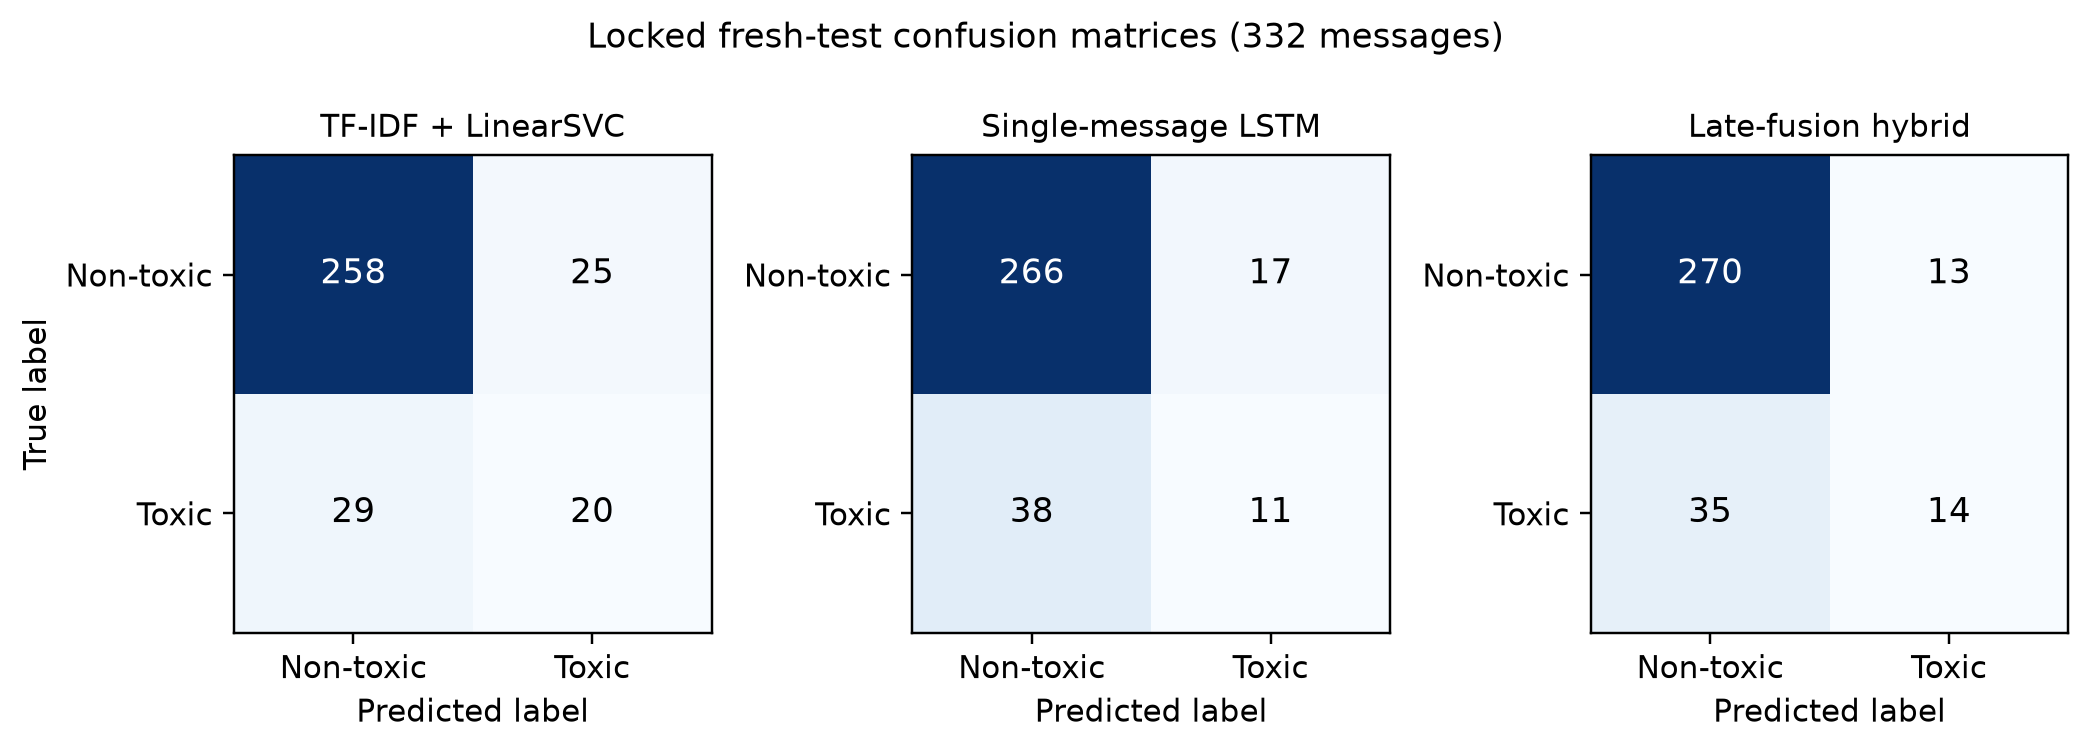
\includegraphics[width=0.75\textwidth]{fresh_confusion.png}
  \caption{Batch~A confusion matrices. Hybrid false alarms \FreshFalsePositives{}; missed toxic \FreshFalseNegatives{}.}
  \label{fig:freshconfusion}
\end{figure}

\section*{Discussion}

I do not think the primary hybrid performs well enough for real chat moderation. On development it barely beat a strong SVM; on Batch~A that small edge disappeared, and on Batch~B the hybrid got worse still. The honest result is a failed transfer, not a deployable detector.

What went wrong is clearer than ``domain shift'' as a vague excuse. In the 10,050-message training split, phrases that show up a lot in Batch~A errors (\texttt{diff}, \texttt{gg ez}, \texttt{skill issue}, \texttt{dogwater}, \texttt{hardstuck}, \texttt{clown}, \texttt{monkey}, \texttt{braindead}, \texttt{touch grass}, \texttt{gap}, \texttt{kys}) each appear zero times, while \texttt{noob} (128 rows, 96\% toxic) and \texttt{stfu} (35 rows, 97\% toxic) are common. My labelling rule also differs from L2DTnH: I mark game sarcasm like ``GG EZ'' toxic and untargeted frustration like ``fuck this game'' non-toxic, while L2DTnH almost always treats \texttt{stfu}-style swearing as toxic. So the model over-flags familiar swear words and under-flags modern put-downs it never saw. Character $n$-grams helped on validation, but Batch~B shows that was not enough for live chat. Covering current slang and matching the label definition matter more here than stacking another neural trick. The project is still hard in a fair way: short imbalanced chat, no public API for text, and OCR-labelled fresh matches. Poor fresh performance is disappointing, but it is explained by the data gap rather than a broken training loop.

\section*{Ethical Considerations}

Wrong toxic flags can punish players, and missed harassment leaves people unprotected. Both errors matter here because my hybrid already makes both kinds of mistakes. Labels are subjective, and slang changes with every patch. Fresh-test labels are from two annotators with a written rubric and no agreement check, so edge cases are uncertain. The OCR collector only looks at voluntarily supplied local match windows and strips identifiers, but any real deployment would still need human review, clear appeals, and ongoing re-labelling rather than silent automatic bans.

{\small\noindent\textit{AI use:} Cursor agents assisted with code, figures, and editing. Metrics come from repository scripts checked against saved result files.}

\clearpage
\section*{Appendix}
\label{app:extra}

Figure~\ref{fig:curves} shows the seed-42 LSTM backbone training curves used by both frozen hybrids. Figure~\ref{fig:batchbconfusion} shows the locked Batch~B confusion matrices for the SVM, LSTM, and character-$n$-gram late-fusion hybrid after thresholds were frozen on validation.

\begin{figure}[!ht]
  \centering
  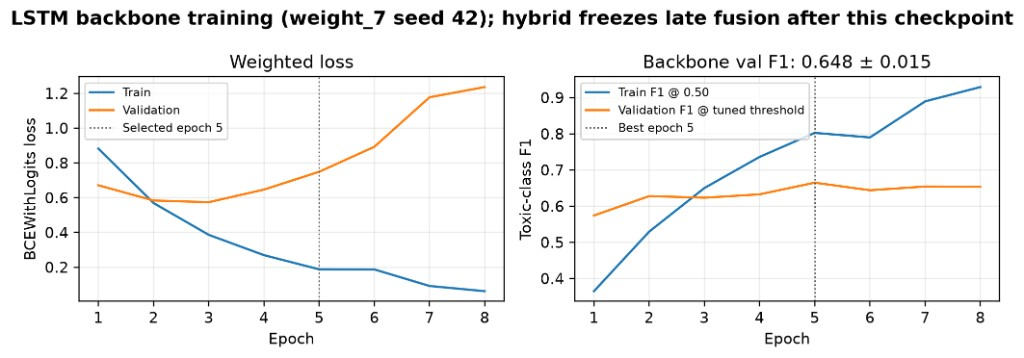
\includegraphics[width=0.92\textwidth]{learning_curves.png}
  \caption{LSTM training (seed 42): best epoch \HybridBestEpoch{} by validation toxic F1; growing train/val loss gap shows overfitting on short chat.}
  \label{fig:curves}
\end{figure}

\begin{figure}[!ht]
  \centering
  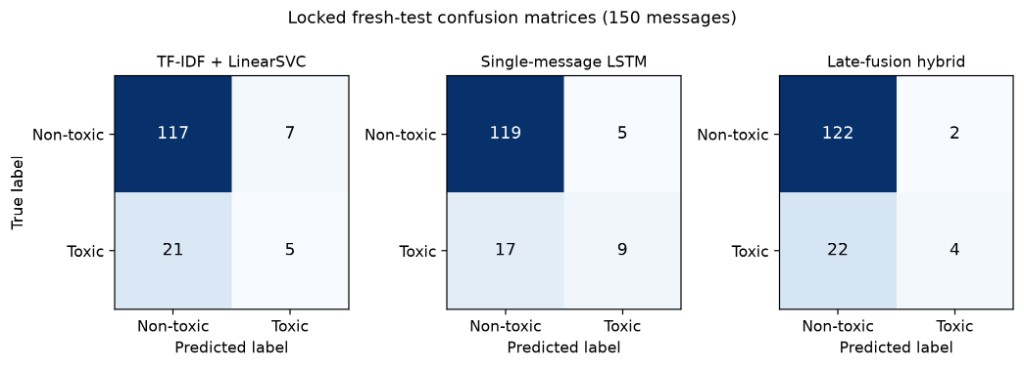
\includegraphics[width=0.98\textwidth]{batch_b_confusion.png}
  \caption{Batch~B confusion matrices (\BatchBMessages{} messages / \BatchBMatches{} matches). Hybrid true positives 4 of \BatchBToxic{}; false negatives 22.}
  \label{fig:batchbconfusion}
\end{figure}

\clearpage
\bibliographystyle{IEEEtran}
\bibliography{references}

\end{document}
